%-----------------------------------------

\subsection{General Remarks}

%-----------------------------------------

\begin{frame}

\frametitle{Theory}
\framesubtitle{Basics}

The goal of \textbf{context generation} and \textbf{contextual bandit algorithms} is to employ a (partially) disaggregated approach in order to better exploit the differences of the users that belong to different classes.

This is made possible by using a specialized Learner for each context and an \textit{offline context generation algorithm} that decides which contexts are worth to target by isolating them from the aggregated data. This algorithm is ran every two weeks.

Each context is able to target a set of features, and a \textbf{context structure} is a set of contexts that targets all the existing features without any overlap.

\end{frame}

%-----------------------------------------

\subsection{Assumptions}

%-----------------------------------------

\begin{frame}

\frametitle{Implementation challenges}
\framesubtitle{Weaknesses}

Context generation has been, by far, the \textit{toughest} task that we faced on this whole project.

Even after many meetings and discussions we felt that there was something that didn't click with our interpretation since we didn't find a way to give a complete meaning to the dataset collected by our active bandits due to how the prediction and the rewards worked in our scenario.

In the end, our final results for this step were \textbf{unsatisfactory} and there is still wide room for improvement.

\end{frame}

%-----------------------------------------

\begin{frame}

\frametitle{Implementation assumptions}
\framesubtitle{Compromises}

Given the difficulties that we encountered, we decided to make some compromises in order to still carry out the task to an end:

\begin{itemize}[label={-}]
    \item The e-commerce website company owns a simulation capable of simulating interactions.
    \item Learners are trained on the fake simulation since we can't get enough information from the logs.
    \item The best expected reward for a given context is considered as the maximum reward experienced by a learner on a fake simulation run.
\end{itemize}

\end{frame}

%-----------------------------------------

\begin{frame}

\frametitle{Implementation assumptions}
\framesubtitle{Potential problems}

Given our interpretation, some quantities were particularly difficult to identify in a correct manner, especially the \textbf{expected value $\mu$ of the optimal arm $a^*$ for a context $c$} (written as $\mu_c$) that we resorted to calculate as the mean reward over a fake simulation on the context $c$.

Additionaly we used the \textbf{Hoeffding bound} to compute lower bounds for both the \textit{context probability} and the \textit{context expected value}.

These particular points are critical parts that absolutely need to be revisioned and most definetly are concurring causes to the unsatisfactory results.

\end{frame}

%-----------------------------------------

\subsection{Implementation}

%-----------------------------------------

\begin{frame}

\frametitle{Greedy algorithm}
\framesubtitle{Part 1 of 2}

We generate contexts following a \textbf{greedy algorithm} that, given a context $c$:

\begin{itemize}[label={*}]
    \item Considers all the possible binary 1-feature splits $\{c_i^0$, $c_i^1\}_n$ for the features not present in $c$.
    \item Creates and evaluates a new learner for each split $c_i^j$, obtaining the \textbf{context probability} $p_i^j$ and the \textbf{best expected reward} $\mu_i^j$.
    \item[] $\rightarrow$
\end{itemize}

\end{frame}

%-----------------------------------------

\begin{frame}

\frametitle{Greedy algorithm}
\framesubtitle{Part 2 of 2}

\begin{itemize}[label={*}]
    \item[] $\rightarrow$
    \item Evaluates the \textbf{splitting condition} on each couple of splits $(c_i^0$, $c_i^1)$ w.r.t the original context $c$ while deciding which split is the best one (if it exists).
    \item If a split has been made, repeat all the operations recursively on the new contexts until \textit{no split is made} or \textit{no split is possible}.
\end{itemize}

\end{frame}

%-----------------------------------------

\begin{frame}

\frametitle{Context generation}
\framesubtitle{Split condition}

Since utilizing multiple contexts is an expensive operation and our \textit{greedy algorithm} is \textbf{not} guranteed to find the optimal solution, we want to be sure that when we introuduce new contexts, it is actually worth to do so.

We use a particular \textit{splitting condition} that exploits lower bounds in order to set a higher threshold for the quality of our splits:

\begin{Large}
    \begin{displaymath}
        \underline{p}_i^0 \underline{\mu}_i^0 + \underline{p}_i^1 \underline{\mu}_i^1 \geq \underline{\mu}_i
    \end{displaymath}
\end{Large}

for context $i$ defined by a binary feature split on 0 and 1.

\end{frame}

%-----------------------------------------

\begin{frame}

\frametitle{Context utilization}

Once a certain number of contexts has been established, a \textbf{Contextual Learner} will be able to assign an \textbf{AlphaUnitless Learner} to each context and obtain their raw predictions by utilizing the function \textbf{predict\_raw} (which returns an un-optimized array of predictions) and then running the optimization algorithm on all the predictions gathered this way.

The resulting \textit{superarm} is then passed to the \textbf{Simulation} which, in return, generates the interactions for the day by weighting the different classes according to the disaggregated predictions.

\end{frame}

%-----------------------------------------

\subsection{Results}

% ----------------------------------------

\begin{frame}[plain]

\frametitle{Reward and regret}
\framesubtitle{Contextual learner}

\begin{center}
    \hspace*{-2.8em}
    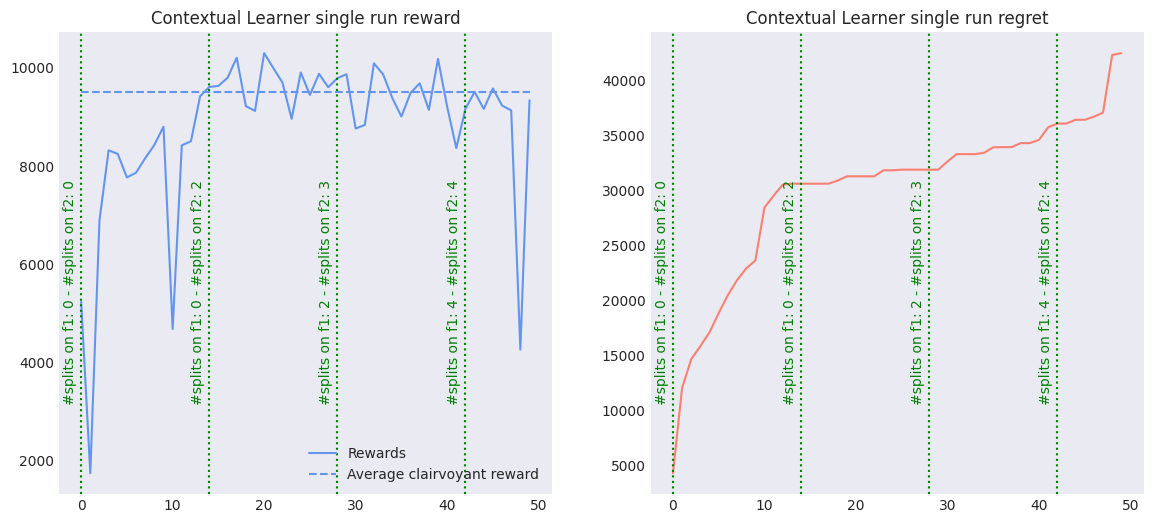
\includegraphics[scale=0.43]{img/Graphs/context_generation/image1.png}
\end{center}

\end{frame}

% ----------------------------------------

\begin{frame}[plain]

\frametitle{Average reward and regret}
\framesubtitle{Contextual learner}

\begin{center}
    \hspace*{-2.8em}
    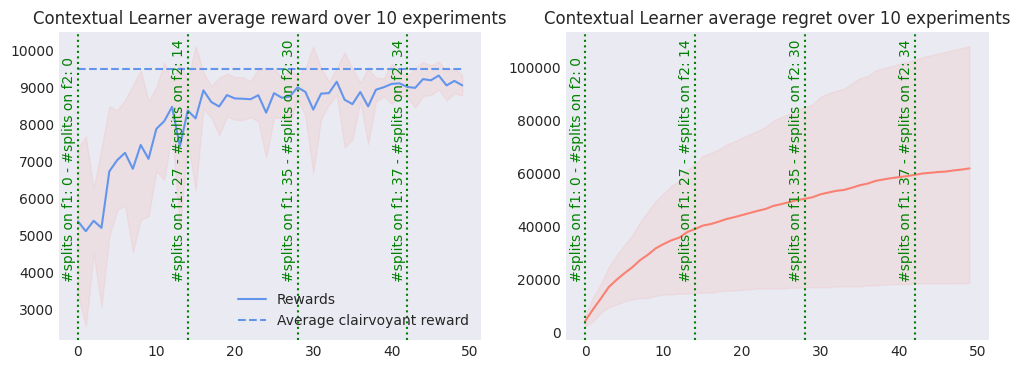
\includegraphics[scale=0.49]{img/Graphs/context_generation/image2.png}
\end{center}

\vspace*{2em}

\scriptsize All tests are done using the \texttt{example\_environment} default values, \textit{population mean} of 800, \textit{variance} of 10 and 20 \textit{budget steps}. Only \textbf{TS} algorithms were evaluated.

\end{frame}

% ----------------------------------------

\begin{frame}

\frametitle{Results}

Even though the results might not be completely satisfying as we would expect a performance superior w.r.t. the \textit{clairvoyant estimation}, on average we still perform better than the \textbf{AlphaUnitLess learner} as we seem to converge to the optimal superarm for the aggregated contexts.

Overall the learners seem to prefer \textbf{early splitting} but various parameters can be tuned (e.g. bound confidence) to make the process of splitting on contexts more \textit{rigorous}.

Average results over 30 runs at time horizon $T = 50$:

\begin{table}
    \begin{tabular}{|c|cc|c|}
    \hline \hline
        \cellcolor{blue!25} & Reward 	& Regret	& Deviation \\
    \cline{2-4}
        \cellcolor{blue!25} & $\mu$		& $\mu$		& $\sigma$	\\
    \hline \hline
        Contextual learner	& 9065.30	& 61719.2	&  273.67	\\
    \hline \hline
    \end{tabular}
\end{table}

\end{frame}

% ----------------------------------------
